\documentclass[a4paper]{ctexart}
	\usepackage{geometry}
	\usepackage{ulem}
	\usepackage{tkz-graph}
	\usepackage{caption}
	\geometry{left=2.54cm,right=2.54cm,top=2.54cm,bottom=2.3cm}
	\title{Day 2题解报告}
	\author{2014060105005{ }何柱{ }男}
\begin{document}
	\maketitle
	\appendix
	\section{Sphinx}
	利用Kruskal算法和并查集。先将所有optical fiber按cost从小到大排序,遍历optical fiber,如果当前的optical fiber连接的两个farm未连通(使用并查集),则添加当前的optical fiber,否则不做处理,遍历结束时所有添加的optical fiber的cost的总和为output。
	\begin{center}
	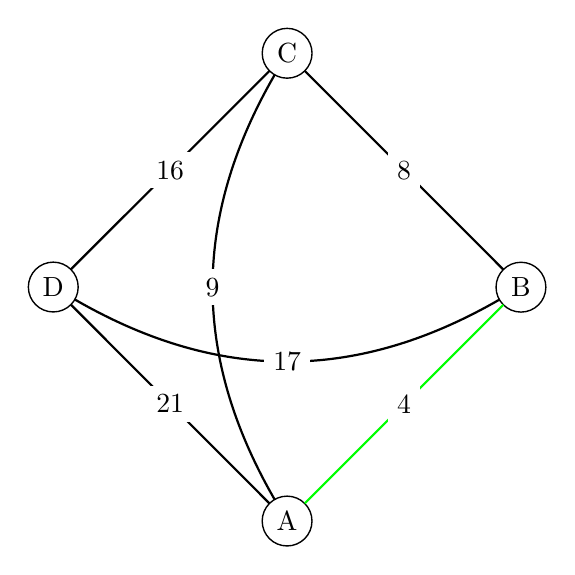
\begin{tikzpicture}[scale=0.8]
	\Vertices[unit=5.25cm]{square}{A,B,C,D}
	\tikzstyle{EdgeStyle}=[green]
	\Edge[label=$4$](A)(B)
	\tikzstyle{EdgeStyle}=[]
	\Edge[label=$8$](B)(C)
	\Edge[label=$16$](C)(D)
	\Edge[label=$21$](D)(A)
	\tikzstyle{EdgeStyle}=[bend left]
	\Edge[label=$9$](A)(C)
	\Edge[label=$17$](B)(D)
	\end{tikzpicture}
	\hspace{0.6cm}
	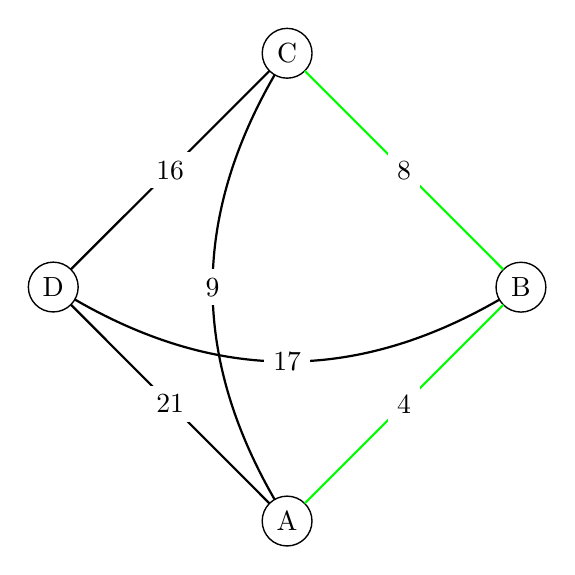
\begin{tikzpicture}[scale=0.8]
	\Vertices[unit=5.25cm]{square}{A,B,C,D}
	\tikzstyle{EdgeStyle}=[green]
	\Edge[label=$4$](A)(B)
	\Edge[label=$8$](B)(C)
	\tikzstyle{EdgeStyle}=[]
	\Edge[label=$16$](C)(D)
	\Edge[label=$21$](D)(A)
	\tikzstyle{EdgeStyle}=[bend left]
	\Edge[label=$9$](A)(C)
	\Edge[label=$17$](B)(D)
	\end{tikzpicture}
	\newline
	\newline
	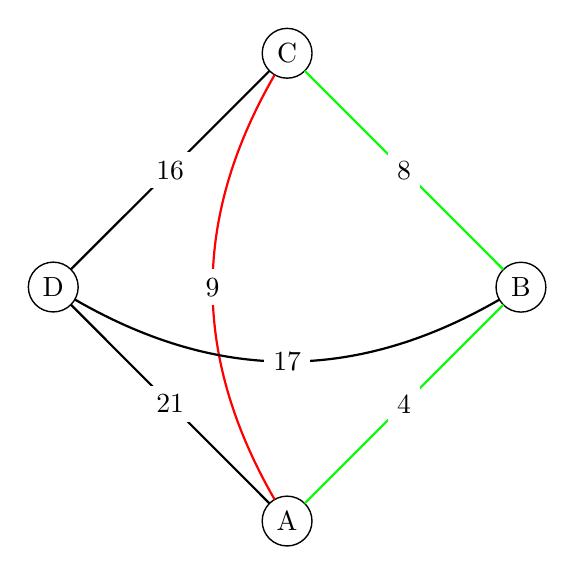
\begin{tikzpicture}[scale=0.8]
	\Vertices[unit=5.25cm]{square}{A,B,C,D}
	\tikzstyle{EdgeStyle}=[green]
	\Edge[label=$4$](A)(B)
	\Edge[label=$8$](B)(C)
	\tikzstyle{EdgeStyle}=[]
	\Edge[label=$16$](C)(D)
	\Edge[label=$21$](D)(A)
	\tikzstyle{EdgeStyle}=[red,bend left]
	\Edge[label=$9$](A)(C)
	\tikzstyle{EdgeStyle}=[bend left]
	\Edge[label=$17$](B)(D)
	\end{tikzpicture}
	\hspace{0.6cm}
	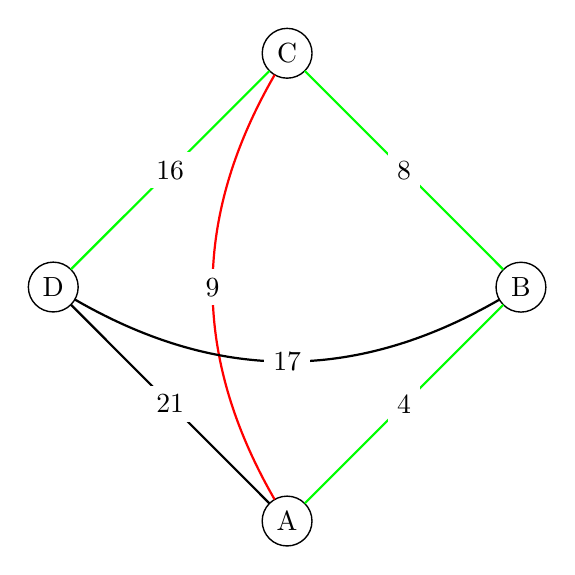
\begin{tikzpicture}[scale=0.8,]
	\Vertices[unit=5.25cm]{square}{A,B,C,D}
	\tikzstyle{EdgeStyle}=[green]
	\Edge[label=$4$](A)(B)
	\Edge[label=$8$](B)(C)
	\Edge[label=$16$](C)(D)
	\tikzstyle{EdgeStyle}=[]
	\Edge[label=$21$](D)(A)
	\tikzstyle{EdgeStyle}=[red,bend left]
	\Edge[label=$9$](A)(C)
	\tikzstyle{EdgeStyle}=[bend left]
	\Edge[label=$17$](B)(D)
	\end{tikzpicture}
	\newline
	\newline
	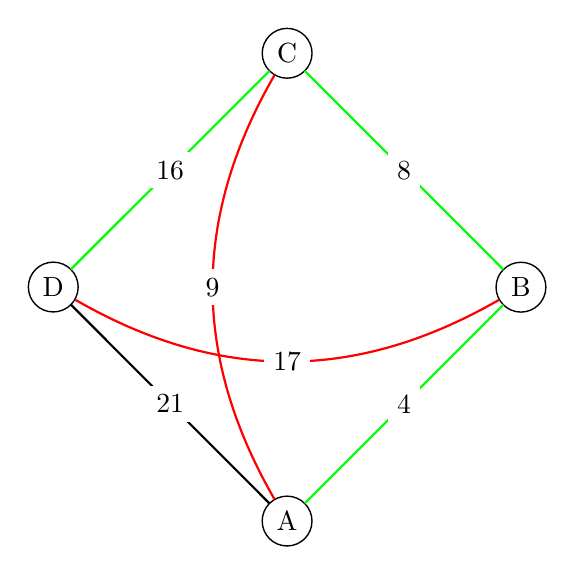
\begin{tikzpicture}[scale=0.8]
	\Vertices[unit=5.25cm]{square}{A,B,C,D}
	\tikzstyle{EdgeStyle}=[green]
	\Edge[label=$4$](A)(B)
	\Edge[label=$8$](B)(C)
	\Edge[label=$16$](C)(D)
	\tikzstyle{EdgeStyle}=[]
	\Edge[label=$21$](D)(A)
	\tikzstyle{EdgeStyle}=[red,bend left]
	\Edge[label=$9$](A)(C)
	\Edge[label=$17$](B)(D)
	\end{tikzpicture}
	\hspace{0.6cm}
	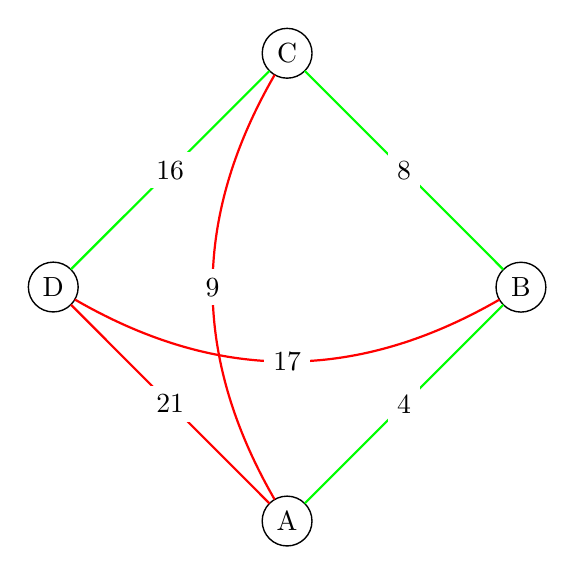
\begin{tikzpicture}[scale=0.8]
	\Vertices[unit=5.25cm]{square}{A,B,C,D}
	\tikzstyle{EdgeStyle}=[green]
	\Edge[label=$4$](A)(B)
	\Edge[label=$8$](B)(C)
	\Edge[label=$16$](C)(D)
	\tikzstyle{EdgeStyle}=[red]
	\Edge[label=$21$](D)(A)
	\tikzstyle{EdgeStyle}=[red,bend left]
	\Edge[label=$9$](A)(C)
	\Edge[label=$17$](B)(D)
	\end{tikzpicture}
	\end{center}
	\setcounter{section}{3}
	\section{Cerberus}
	\begin{enumerate}
		\item 建立带延迟标记的线段树:让根节点表示区间$[0,N)$,把区间分两半,分别由左右子树表示,再将子树做相似的处理。每个节点包含区间的总和与延迟标记(初始值为0)。
		\item 查询$[A,B)$的总和:从根节点开始查询,如果节点包含于区间内,返回节点的值;如果节点与区间有交集,(如果节点有标记,把标记传到子树上,并把标记应用到子树的值上),查询左右子树的节点;否则返回0。
		\item 更新$[A,B)$:从根节点开始更新,如果节点包含于区间内,把值加到节点的值上和标记上;如果节点与区间有交集,(如果节点有标记,把标记传到子树上,并把标记应用到子树的值上),更新左右子树的节点。
	\end{enumerate}
	\begin{center}
	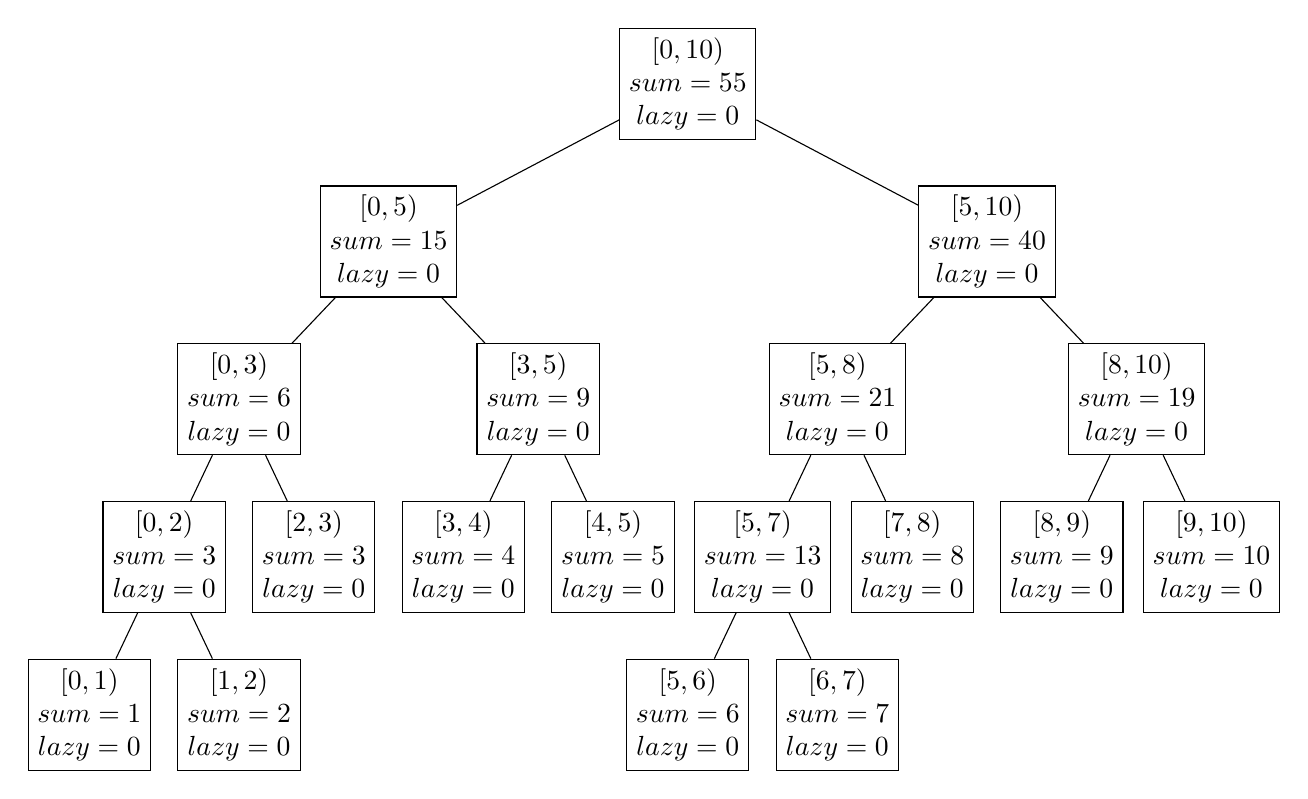
\begin{tikzpicture}[scale=0.95]
	\node [draw, align=center]{$[0,10)$ \\ $sum=55$ \\ $lazy=0$}
	[sibling distance=8cm]
	[level distance=60pt]
	child {node [draw, align=center]{$[0,5)$ \\ $sum=15$ \\ $lazy=0$}
		[sibling distance=4cm]
	    child {node [draw, align=center]{$[0,3)$ \\ $sum=6$ \\ $lazy=0$}
			[sibling distance=2cm]
			child {node [draw, align=center]{$[0,2)$ \\ $sum=3$ \\ $lazy=0$}
				[sibling distance=2cm]
			    child {node [draw, align=center]{$[0,1)$ \\ $sum=1$ \\ $lazy=0$}}
			    child {node [draw, align=center]{$[1,2)$ \\ $sum=2$ \\ $lazy=0$}}
			}
	   		child {node [draw, align=center]{$[2,3)$ \\ $sum=3$ \\ $lazy=0$}}
	    }
	    child {node [draw, align=center]{$[3,5)$ \\ $sum=9$ \\ $lazy=0$}
			[sibling distance=2cm]
			child {node [draw, align=center]{$[3,4)$ \\ $sum=4$ \\ $lazy=0$}}
	   		child {node [draw, align=center]{$[4,5)$ \\ $sum=5$ \\ $lazy=0$}}
	    }
	}
	child {node [draw, align=center]{$[5,10)$ \\ $sum=40$ \\ $lazy=0$}
		[sibling distance=4cm]
	    child {node [draw, align=center]{$[5,8)$ \\ $sum=21$ \\ $lazy=0$}
			[sibling distance=2cm]
			child {node [draw, align=center]{$[5,7)$ \\ $sum=13$ \\ $lazy=0$}
				[sibling distance=2cm]
			    child {node [draw, align=center]{$[5,6)$ \\ $sum=6$ \\ $lazy=0$}}
			    child {node [draw, align=center]{$[6,7)$ \\ $sum=7$ \\ $lazy=0$}}
			}
	   		child {node [draw, align=center]{$[7,8)$ \\ $sum=8$ \\ $lazy=0$}}
	    }
	    child {node [draw, align=center]{$[8,10)$ \\ $sum=19$ \\ $lazy=0$}
			[sibling distance=2cm]
			child {node [draw, align=center]{$[8,9)$ \\ $sum=9$ \\ $lazy=0$}}
	   		child {node [draw, align=center]{$[9,10)$ \\ $sum=10$ \\ $lazy=0$}}
	    }
	};
	\end{tikzpicture}
	\captionof{figure}{建立带延迟标记的线段树}
	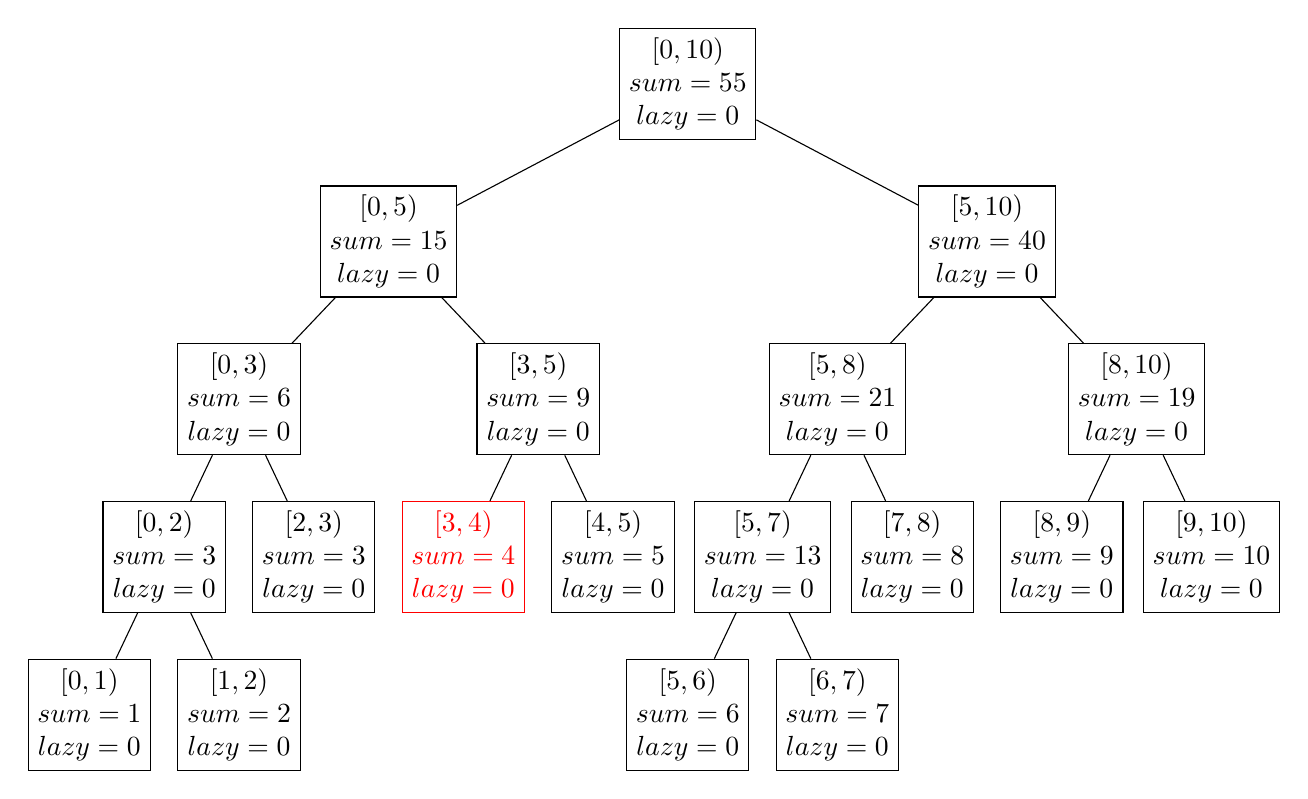
\begin{tikzpicture}[scale=0.95]
	\node [draw, align=center]{$[0,10)$ \\ $sum=55$ \\ $lazy=0$}
	[sibling distance=8cm]
	[level distance=60pt]
	child {node [draw, align=center]{$[0,5)$ \\ $sum=15$ \\ $lazy=0$}
		[sibling distance=4cm]
	    child {node [draw, align=center]{$[0,3)$ \\ $sum=6$ \\ $lazy=0$}
			[sibling distance=2cm]
			child {node [draw, align=center]{$[0,2)$ \\ $sum=3$ \\ $lazy=0$}
				[sibling distance=2cm]
			    child {node [draw, align=center]{$[0,1)$ \\ $sum=1$ \\ $lazy=0$}}
			    child {node [draw, align=center]{$[1,2)$ \\ $sum=2$ \\ $lazy=0$}}
			}
	   		child {node [draw, align=center]{$[2,3)$ \\ $sum=3$ \\ $lazy=0$}}
	    }
	    child {node [draw, align=center]{$[3,5)$ \\ $sum=9$ \\ $lazy=0$}
			[sibling distance=2cm]
			child {node [draw, align=center, red]{$[3,4)$ \\ $sum=4$ \\ $lazy=0$}}
	   		child {node [draw, align=center]{$[4,5)$ \\ $sum=5$ \\ $lazy=0$}}
	    }
	}
	child {node [draw, align=center]{$[5,10)$ \\ $sum=40$ \\ $lazy=0$}
		[sibling distance=4cm]
	    child {node [draw, align=center]{$[5,8)$ \\ $sum=21$ \\ $lazy=0$}
			[sibling distance=2cm]
			child {node [draw, align=center]{$[5,7)$ \\ $sum=13$ \\ $lazy=0$}
				[sibling distance=2cm]
			    child {node [draw, align=center]{$[5,6)$ \\ $sum=6$ \\ $lazy=0$}}
			    child {node [draw, align=center]{$[6,7)$ \\ $sum=7$ \\ $lazy=0$}}
			}
	   		child {node [draw, align=center]{$[7,8)$ \\ $sum=8$ \\ $lazy=0$}}
	    }
	    child {node [draw, align=center]{$[8,10)$ \\ $sum=19$ \\ $lazy=0$}
			[sibling distance=2cm]
			child {node [draw, align=center]{$[8,9)$ \\ $sum=9$ \\ $lazy=0$}}
	   		child {node [draw, align=center]{$[9,10)$ \\ $sum=10$ \\ $lazy=0$}}
	    }
	};
	\end{tikzpicture}
	\captionof{figure}{Q 4 4}
	\end{center}
	\begin{center}
	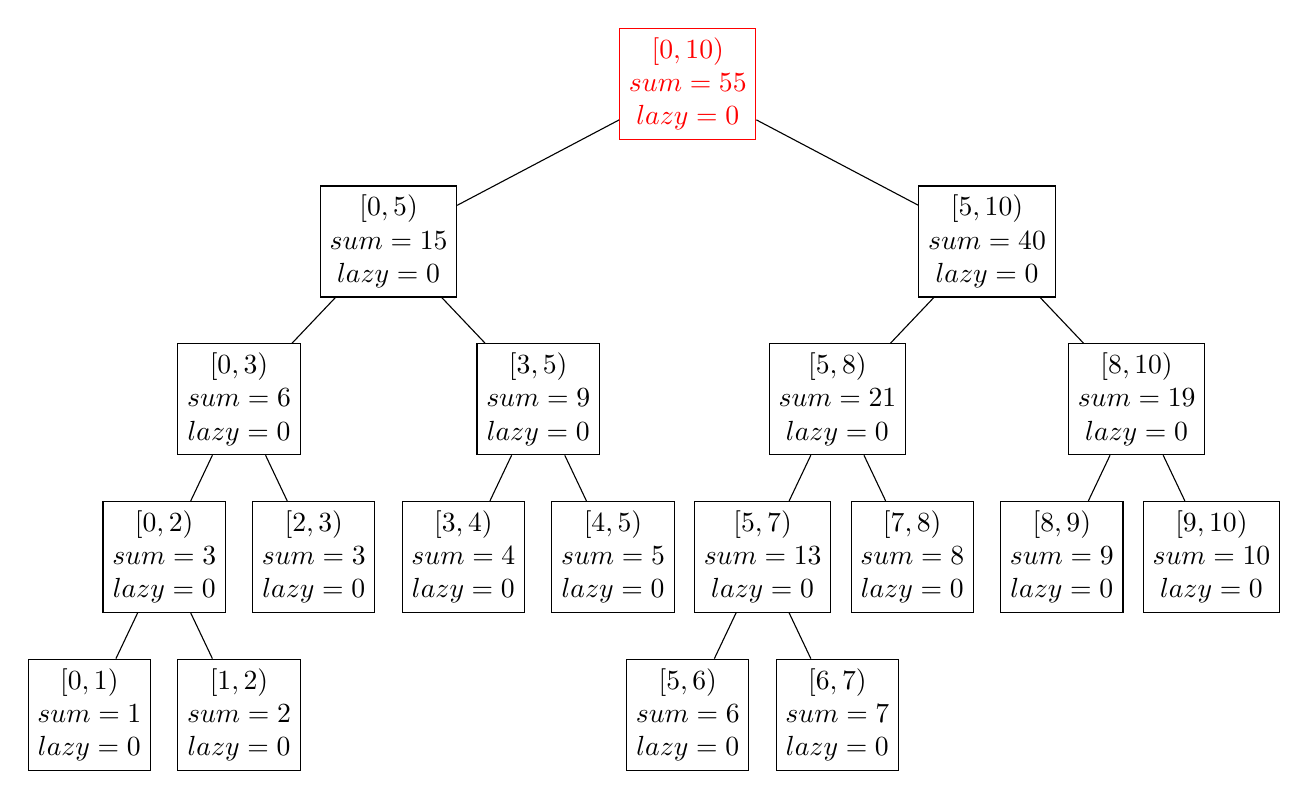
\begin{tikzpicture}[scale=0.95]
	\node [draw, align=center, red]{$[0,10)$ \\ $sum=55$ \\ $lazy=0$}
	[sibling distance=8cm]
	[level distance=60pt]
	child {node [draw, align=center]{$[0,5)$ \\ $sum=15$ \\ $lazy=0$}
		[sibling distance=4cm]
	    child {node [draw, align=center]{$[0,3)$ \\ $sum=6$ \\ $lazy=0$}
			[sibling distance=2cm]
			child {node [draw, align=center]{$[0,2)$ \\ $sum=3$ \\ $lazy=0$}
				[sibling distance=2cm]
			    child {node [draw, align=center]{$[0,1)$ \\ $sum=1$ \\ $lazy=0$}}
			    child {node [draw, align=center]{$[1,2)$ \\ $sum=2$ \\ $lazy=0$}}
			}
	   		child {node [draw, align=center]{$[2,3)$ \\ $sum=3$ \\ $lazy=0$}}
	    }
	    child {node [draw, align=center]{$[3,5)$ \\ $sum=9$ \\ $lazy=0$}
			[sibling distance=2cm]
			child {node [draw, align=center]{$[3,4)$ \\ $sum=4$ \\ $lazy=0$}}
	   		child {node [draw, align=center]{$[4,5)$ \\ $sum=5$ \\ $lazy=0$}}
	    }
	}
	child {node [draw, align=center]{$[5,10)$ \\ $sum=40$ \\ $lazy=0$}
		[sibling distance=4cm]
	    child {node [draw, align=center]{$[5,8)$ \\ $sum=21$ \\ $lazy=0$}
			[sibling distance=2cm]
			child {node [draw, align=center]{$[5,7)$ \\ $sum=13$ \\ $lazy=0$}
				[sibling distance=2cm]
			    child {node [draw, align=center]{$[5,6)$ \\ $sum=6$ \\ $lazy=0$}}
			    child {node [draw, align=center]{$[6,7)$ \\ $sum=7$ \\ $lazy=0$}}
			}
	   		child {node [draw, align=center]{$[7,8)$ \\ $sum=8$ \\ $lazy=0$}}
	    }
	    child {node [draw, align=center]{$[8,10)$ \\ $sum=19$ \\ $lazy=0$}
			[sibling distance=2cm]
			child {node [draw, align=center]{$[8,9)$ \\ $sum=9$ \\ $lazy=0$}}
	   		child {node [draw, align=center]{$[9,10)$ \\ $sum=10$ \\ $lazy=0$}}
	    }
	};
	\end{tikzpicture}
	\captionof{figure}{Q 1 10}
	\end{center}
	\begin{center}
	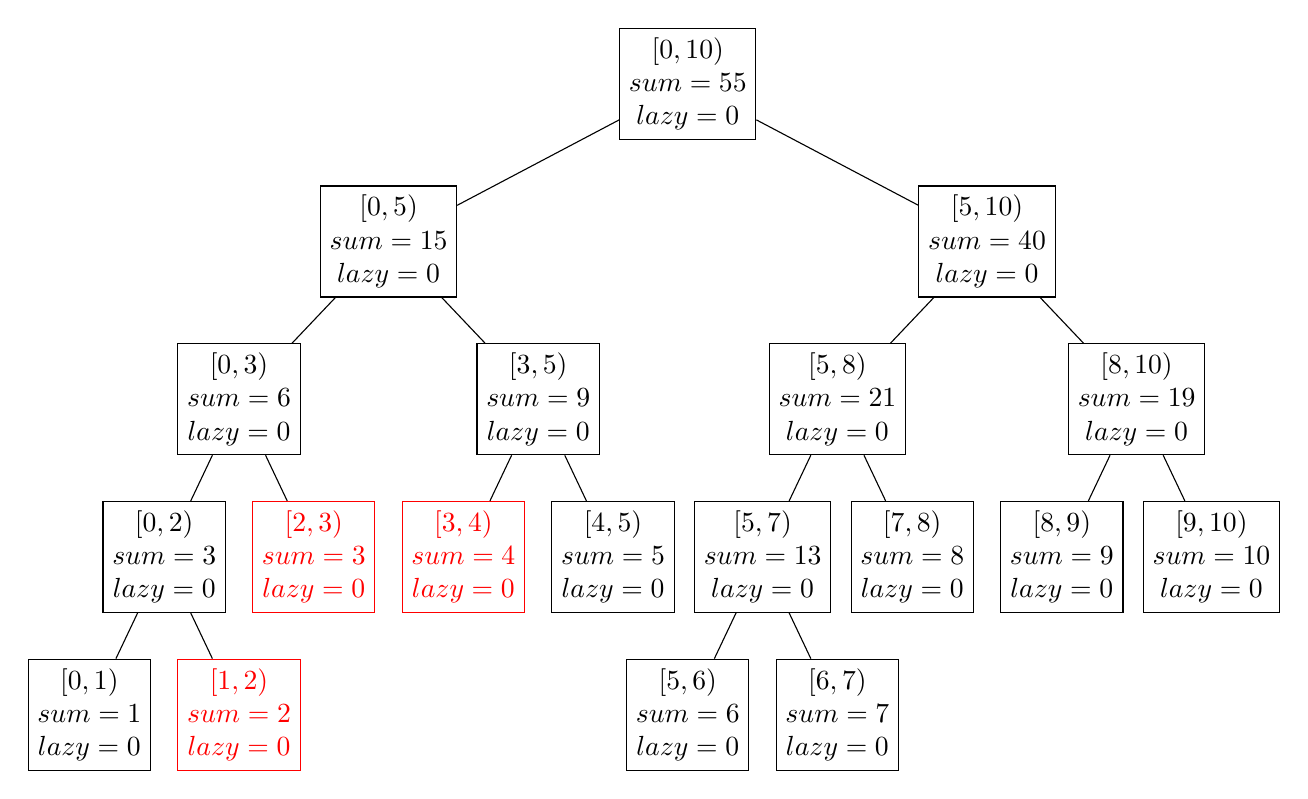
\begin{tikzpicture}[scale=0.95]
	\node [draw, align=center]{$[0,10)$ \\ $sum=55$ \\ $lazy=0$}
	[sibling distance=8cm]
	[level distance=60pt]
	child {node [draw, align=center]{$[0,5)$ \\ $sum=15$ \\ $lazy=0$}
		[sibling distance=4cm]
	    child {node [draw, align=center]{$[0,3)$ \\ $sum=6$ \\ $lazy=0$}
			[sibling distance=2cm]
			child {node [draw, align=center]{$[0,2)$ \\ $sum=3$ \\ $lazy=0$}
				[sibling distance=2cm]
			    child {node [draw, align=center]{$[0,1)$ \\ $sum=1$ \\ $lazy=0$}}
			    child {node [draw, align=center, red]{$[1,2)$ \\ $sum=2$ \\ $lazy=0$}}
			}
	   		child {node [draw, align=center, red]{$[2,3)$ \\ $sum=3$ \\ $lazy=0$}}
	    }
	    child {node [draw, align=center]{$[3,5)$ \\ $sum=9$ \\ $lazy=0$}
			[sibling distance=2cm]
			child {node [draw, align=center, red]{$[3,4)$ \\ $sum=4$ \\ $lazy=0$}}
	   		child {node [draw, align=center]{$[4,5)$ \\ $sum=5$ \\ $lazy=0$}}
	    }
	}
	child {node [draw, align=center]{$[5,10)$ \\ $sum=40$ \\ $lazy=0$}
		[sibling distance=4cm]
	    child {node [draw, align=center]{$[5,8)$ \\ $sum=21$ \\ $lazy=0$}
			[sibling distance=2cm]
			child {node [draw, align=center]{$[5,7)$ \\ $sum=13$ \\ $lazy=0$}
				[sibling distance=2cm]
			    child {node [draw, align=center]{$[5,6)$ \\ $sum=6$ \\ $lazy=0$}}
			    child {node [draw, align=center]{$[6,7)$ \\ $sum=7$ \\ $lazy=0$}}
			}
	   		child {node [draw, align=center]{$[7,8)$ \\ $sum=8$ \\ $lazy=0$}}
	    }
	    child {node [draw, align=center]{$[8,10)$ \\ $sum=19$ \\ $lazy=0$}
			[sibling distance=2cm]
			child {node [draw, align=center]{$[8,9)$ \\ $sum=9$ \\ $lazy=0$}}
	   		child {node [draw, align=center]{$[9,10)$ \\ $sum=10$ \\ $lazy=0$}}
	    }
	};
	\end{tikzpicture}
	\captionof{figure}{Q 2 4}
	\end{center}
	\begin{center}
	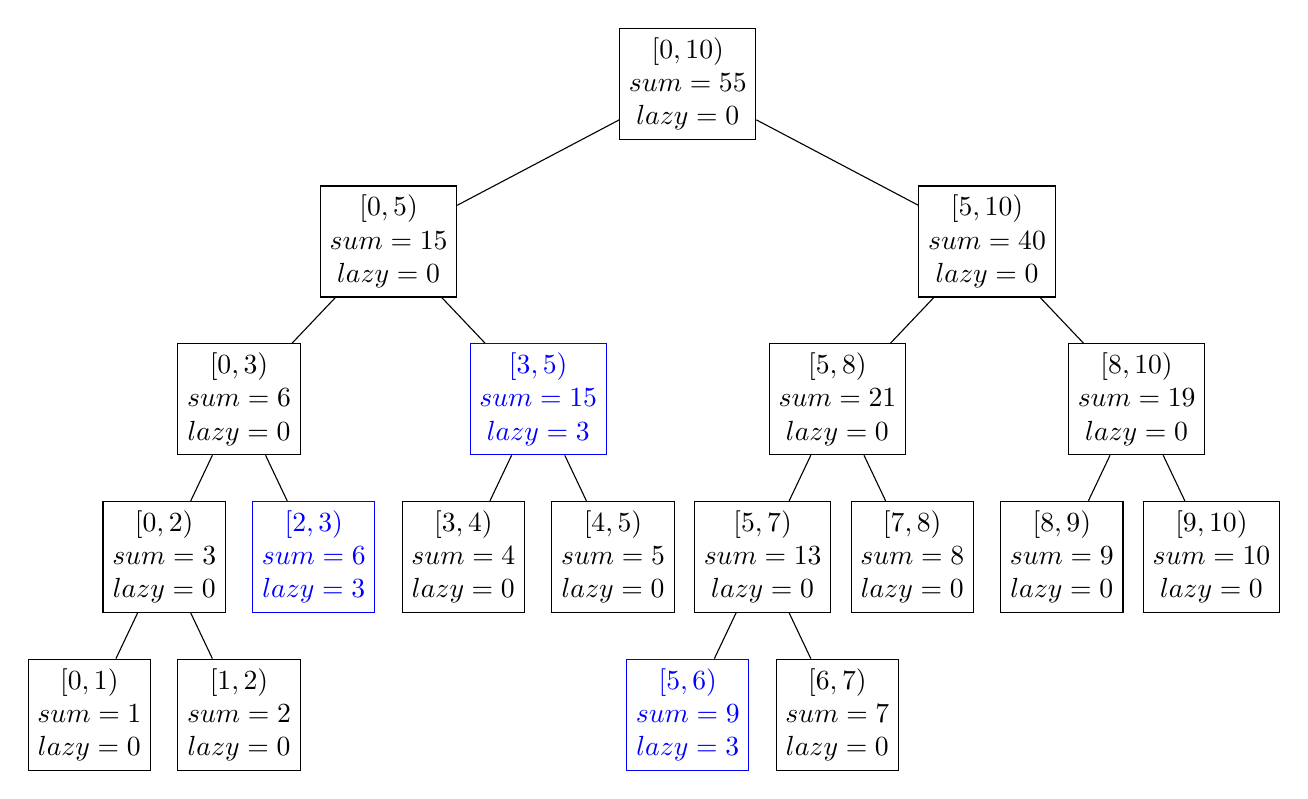
\begin{tikzpicture}[scale=0.95]
	\node [draw, align=center]{$[0,10)$ \\ $sum=55$ \\ $lazy=0$}
	[sibling distance=8cm]
	[level distance=60pt]
	child {node [draw, align=center]{$[0,5)$ \\ $sum=15$ \\ $lazy=0$}
		[sibling distance=4cm]
	    child {node [draw, align=center]{$[0,3)$ \\ $sum=6$ \\ $lazy=0$}
			[sibling distance=2cm]
			child {node [draw, align=center]{$[0,2)$ \\ $sum=3$ \\ $lazy=0$}
				[sibling distance=2cm]
			    child {node [draw, align=center]{$[0,1)$ \\ $sum=1$ \\ $lazy=0$}}
			    child {node [draw, align=center]{$[1,2)$ \\ $sum=2$ \\ $lazy=0$}}
			}
	   		child {node [draw, align=center, blue]{$[2,3)$ \\ $sum=6$ \\ $lazy=3$}}
	    }
	    child {node [draw, align=center, blue]{$[3,5)$ \\ $sum=15$ \\ $lazy=3$}
			[sibling distance=2cm]
			child {node [draw, align=center]{$[3,4)$ \\ $sum=4$ \\ $lazy=0$}}
	   		child {node [draw, align=center]{$[4,5)$ \\ $sum=5$ \\ $lazy=0$}}
	    }
	}
	child {node [draw, align=center]{$[5,10)$ \\ $sum=40$ \\ $lazy=0$}
		[sibling distance=4cm]
	    child {node [draw, align=center]{$[5,8)$ \\ $sum=21$ \\ $lazy=0$}
			[sibling distance=2cm]
			child {node [draw, align=center]{$[5,7)$ \\ $sum=13$ \\ $lazy=0$}
				[sibling distance=2cm]
			    child {node [draw, align=center, blue]{$[5,6)$ \\ $sum=9$ \\ $lazy=3$}}
			    child {node [draw, align=center]{$[6,7)$ \\ $sum=7$ \\ $lazy=0$}}
			}
	   		child {node [draw, align=center]{$[7,8)$ \\ $sum=8$ \\ $lazy=0$}}
	    }
	    child {node [draw, align=center]{$[8,10)$ \\ $sum=19$ \\ $lazy=0$}
			[sibling distance=2cm]
			child {node [draw, align=center]{$[8,9)$ \\ $sum=9$ \\ $lazy=0$}}
	   		child {node [draw, align=center]{$[9,10)$ \\ $sum=10$ \\ $lazy=0$}}
	    }
	};
	\end{tikzpicture}
	\captionof{figure}{C 3 6 3}
	\end{center}
	\begin{center}
	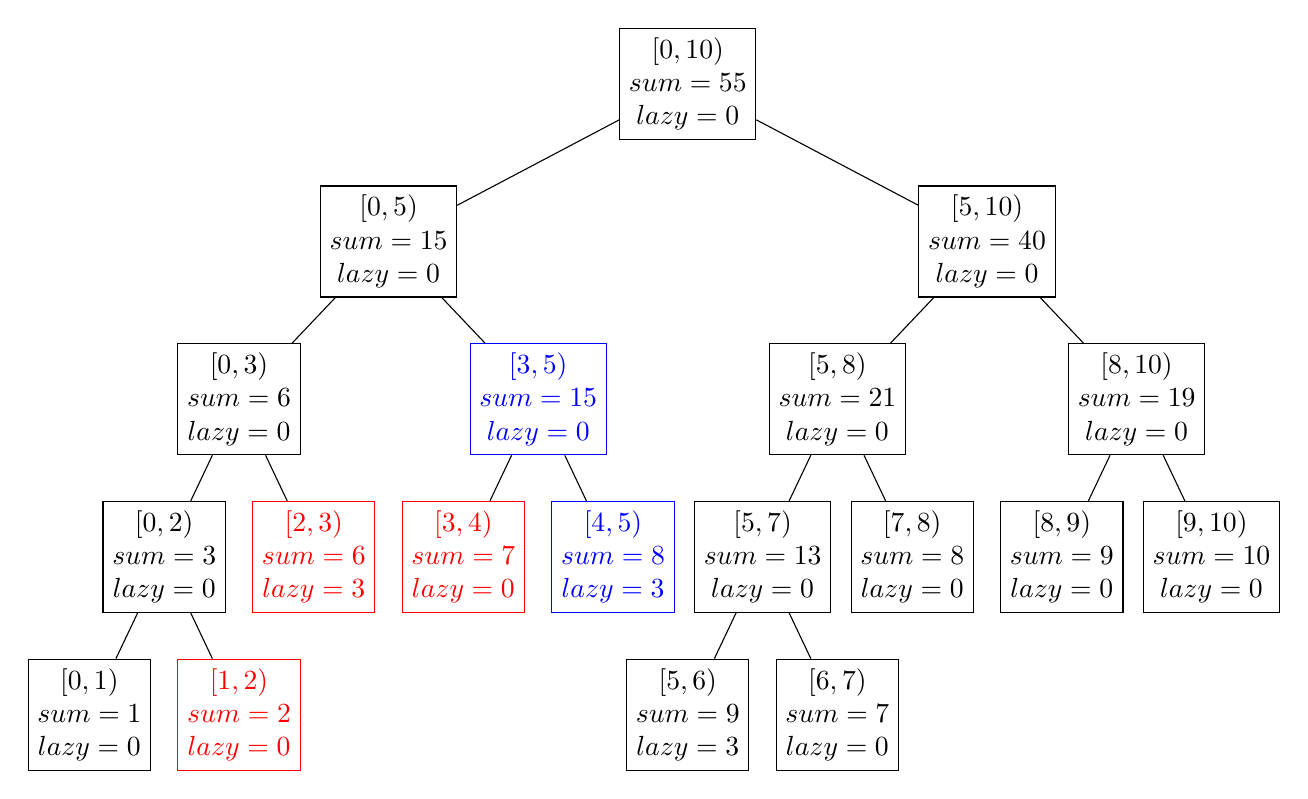
\begin{tikzpicture}[scale=0.95]
	\node [draw, align=center]{$[0,10)$ \\ $sum=55$ \\ $lazy=0$}
	[sibling distance=8cm]
	[level distance=60pt]
	child {node [draw, align=center]{$[0,5)$ \\ $sum=15$ \\ $lazy=0$}
		[sibling distance=4cm]
	    child {node [draw, align=center]{$[0,3)$ \\ $sum=6$ \\ $lazy=0$}
			[sibling distance=2cm]
			child {node [draw, align=center]{$[0,2)$ \\ $sum=3$ \\ $lazy=0$}
				[sibling distance=2cm]
			    child {node [draw, align=center]{$[0,1)$ \\ $sum=1$ \\ $lazy=0$}}
			    child {node [draw, align=center, red]{$[1,2)$ \\ $sum=2$ \\ $lazy=0$}}
			}
	   		child {node [draw, align=center, red]{$[2,3)$ \\ $sum=6$ \\ $lazy=3$}}
	    }
	    child {node [draw, align=center, blue]{$[3,5)$ \\ $sum=15$ \\ $lazy=0$}
			[sibling distance=2cm]
			child {node [draw, align=center, red]{$[3,4)$ \\ $sum=7$ \\ $lazy=0$}}
	   		child {node [draw, align=center, blue]{$[4,5)$ \\ $sum=8$ \\ $lazy=3$}}
	    }
	}
	child {node [draw, align=center]{$[5,10)$ \\ $sum=40$ \\ $lazy=0$}
		[sibling distance=4cm]
	    child {node [draw, align=center]{$[5,8)$ \\ $sum=21$ \\ $lazy=0$}
			[sibling distance=2cm]
			child {node [draw, align=center]{$[5,7)$ \\ $sum=13$ \\ $lazy=0$}
				[sibling distance=2cm]
			    child {node [draw, align=center]{$[5,6)$ \\ $sum=9$ \\ $lazy=3$}}
			    child {node [draw, align=center]{$[6,7)$ \\ $sum=7$ \\ $lazy=0$}}
			}
	   		child {node [draw, align=center]{$[7,8)$ \\ $sum=8$ \\ $lazy=0$}}
	    }
	    child {node [draw, align=center]{$[8,10)$ \\ $sum=19$ \\ $lazy=0$}
			[sibling distance=2cm]
			child {node [draw, align=center]{$[8,9)$ \\ $sum=9$ \\ $lazy=0$}}
	   		child {node [draw, align=center]{$[9,10)$ \\ $sum=10$ \\ $lazy=0$}}
	    }
	};
	\end{tikzpicture}
	\captionof{figure}{Q 2 4}
	\end{center}
\end{document}